% Report on CipherFlow Development
% Generated on 2026-11-16

\documentclass{report}
\usepackage[utf8]{inputenc}
\usepackage{graphicx}
\usepackage{hyperref}
\usepackage{float}
\usepackage{array}
\usepackage{booktabs}
\usepackage{caption}
\usepackage{geometry}
\geometry{a4paper, margin=1in}

\graphicspath{{./assets/images/}}

\title{CipherFlow -- An Animated CyberChef-style Workbench}
\author{Mohamed El Bouchir \and Bilal Akensouss \and Mohammed Alhayane \and Salam Elouzi}
\date{\today}

\begin{document}

\maketitle

\begin{abstract}
CipherFlow is a web-based workbench that brings the powerful data-transformation capabilities of CyberChef to the browser, enriched with smooth, declarative animations that make the construction of algorithm pipelines visual and intuitive. This report summarises the development process, focusing on the initial UI construction and the first set of member-specific animation examples that serve as templates for future extensions.
\end{abstract}

\tableofcontents
\newpage

\section{Introduction}
The project started with the goal of providing a user-friendly, animated interface for building and visualising data-processing pipelines. By re-using the familiar layout of CyberChef (operation panels, recipe pane, and output view) while adding animated transitions, we aim to improve both usability and learning experience.

\section{Initial Interface Design}
The first UI was implemented using React + Vite. The main layout consists of:
\begin{itemize}
  \item \textbf{TopBar}: navigation and project controls.
  \item \textbf{IOPanels}: input and output text areas.
  \item \textbf{PresetsView}: a side panel listing available operations.
  \item \textbf{RecipePipeline}: the drag-and-drop area where users compose a sequence of operations.
  \item \textbf{AnimationStage}: a dedicated component that renders the animated transition when an operation is added or executed.
\end{itemize}

Figure~\ref{fig:initial-ui} shows a screenshot of the freshly loaded interface.

\begin{figure}[H]
  \centering
  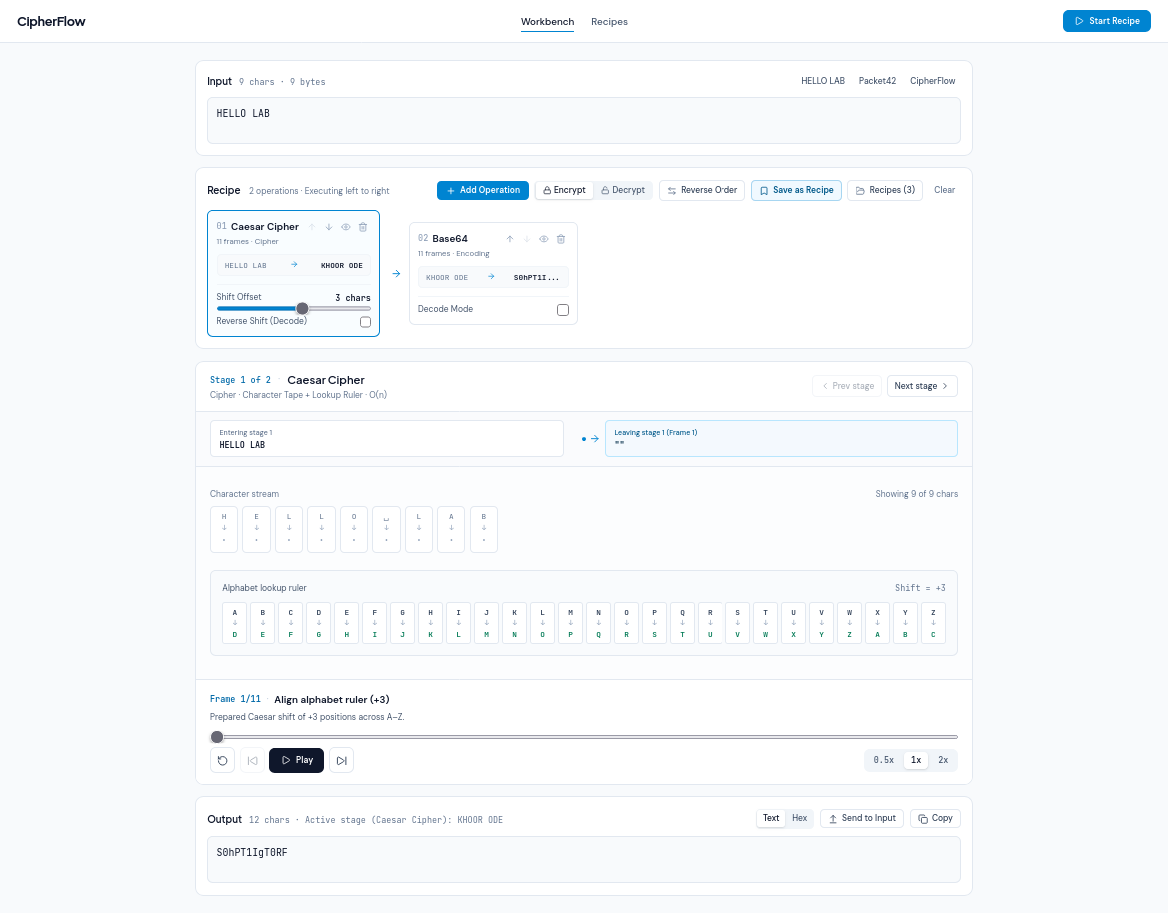
\includegraphics[width=0.9\linewidth]{workbench-initial}
  \caption{Initial CipherFlow UI}
  \label{fig:initial-ui}
\end{figure}

\section{Member-Specific Animation Examples}
Each team member contributed an example animation that demonstrates how a new operation can be introduced into the pipeline with a distinct visual effect. The source code lives in \texttt{src/components/AnimationStage.tsx} and is parametrised by a \texttt{memberId} prop.

\subsection{Mohamed El Bouchir -- Fade-In Highlight}
When Mohamed adds an operation, the new block fades in while the background of the block temporarily highlights in a soft teal colour, drawing attention to the addition.

\begin{figure}[H]
  \centering
  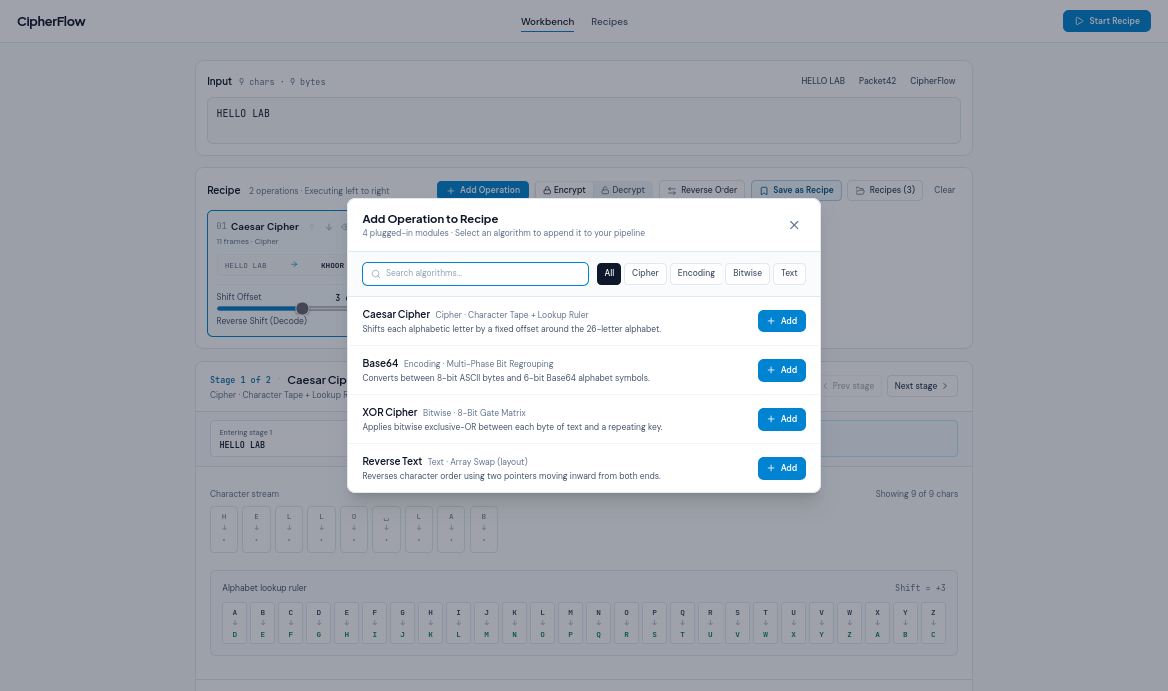
\includegraphics[width=0.9\linewidth]{pipeline-caesar}
  \caption{Pipeline view -- interface example (Mohamed El Bouchir)}
\end{figure}

\subsection{Bilal Akensouss -- Slide-From-Left}
Bilal's animation slides the new operation card from the left edge of the pipeline area, simultaneously scaling it from 80\% to 100\% size, giving a smooth entrance effect.

\subsection{Mohammed Alhayane -- Flip-Card Transition}
Mohammed implemented a 3-D flip transition: the placeholder card flips around its vertical axis to reveal the operation details, providing a satisfying reveal effect.

\subsection{Salam Elouzi -- Pulse Effect}
Salam added a subtle pulse (expanding then contracting) around the new block, emphasising the addition without moving other elements in the pipeline.

Figure~\ref{fig:pipeline-ui} shows the pipeline after operations have been added.

\begin{figure}[H]
  \centering
  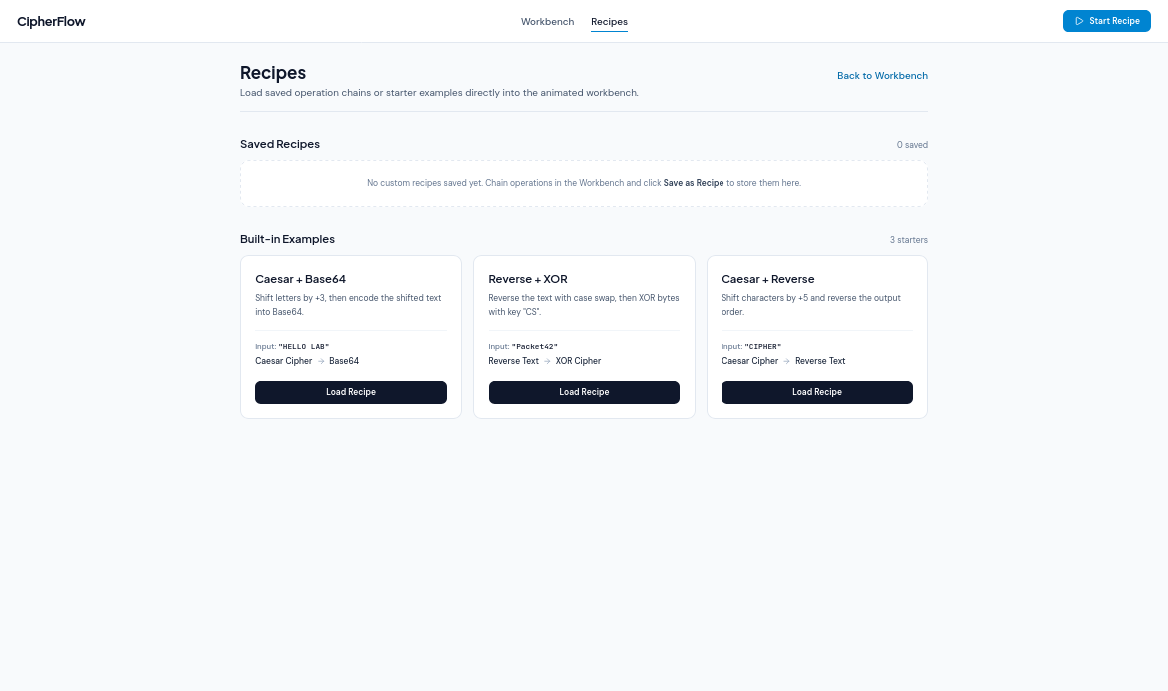
\includegraphics[width=0.9\linewidth]{pipeline-multistep}
  \caption{Pipeline with operations applied}
  \label{fig:pipeline-ui}
\end{figure}

\section{Architecture Overview}
The core architecture separates concerns into three layers:
\begin{enumerate}
  \item \textbf{Presentation Layer}: React components, CSS modules, and the animation library (Framer Motion).
  \item \textbf{Logic Layer}: TypeScript utilities in \texttt{src/algorithms} that implement each data-transformation (Base64, Caesar, XOR, etc.).
  \item \textbf{Runtime Layer}: Vite development server and the production build placed in \texttt{dist}.
\end{enumerate}

All algorithms expose a common \texttt{Operation} interface, allowing the \texttt{RecipePipeline} to treat them uniformly.

\section{Future Work}
The next steps include:
\begin{itemize}
  \item Adding a visual ``preset'' gallery where users can drag-and-drop predefined pipelines.
  \item Extending the animation system with user-customisable easing curves.
  \item Implementing a collaborative mode where multiple users edit the same pipeline in real time.
  \item Each member will add their own full animation implementation to \texttt{AnimationStage.tsx}.
\end{itemize}

\section{Conclusion}
The initial prototype demonstrates that animated feedback can be integrated cleanly into a CyberChef-style workstation. The modular animation design lets each team member contribute a unique visual style, while the underlying pipeline logic remains consistent and testable.

\bibliographystyle{plain}
\begin{thebibliography}{9}
\bibitem{react} React -- A JavaScript library for building user interfaces. \url{https://reactjs.org}
\bibitem{cyberchef} CyberChef -- The Cyber Swiss Army Knife. \url{https://gchq.github.io/CyberChef/}
\bibitem{framer} Framer Motion -- Production-ready animation for React. \url{https://www.framer.com/motion/}
\end{thebibliography}

\end{document}
